\documentclass[tikz,border=4pt]{standalone}
% Shared style for MultiMM figures (white background, logo palette)
\usepackage{tikz,pgfplots,amsmath}
\pgfplotsset{compat=1.16}
\usetikzlibrary{arrows.meta,calc,decorations.pathreplacing,positioning,backgrounds}
\definecolor{indigo}{HTML}{3B37A0}
\definecolor{violet}{HTML}{6A3AA8}
\definecolor{crimson}{HTML}{B5406C}
\definecolor{gold}{HTML}{E9A62C}
\definecolor{golddark}{HTML}{B9791A}
\definecolor{grey}{HTML}{8A8AA0}
\definecolor{lightgrey}{HTML}{E4E4EE}
\tikzset{
  bead/.style={circle,draw=#1!80!black,fill=#1!35,line width=0.5pt,minimum size=9pt,inner sep=0pt},
  bead/.default=indigo,
  lab/.style={font=\small},
}
\pgfplotsset{
  every axis/.append style={
    width=9.5cm,height=6.3cm,axis lines=left,line width=0.5pt,
    grid=major,grid style={draw=lightgrey,line width=0.3pt},
    tick label style={font=\small},label style={font=\normalsize},
    legend style={font=\footnotesize,draw=none,fill=white,fill opacity=0.8,text opacity=1},
    legend cell align=left,
  },
  every axis plot/.append style={line width=1.2pt,smooth},
}

\begin{document}
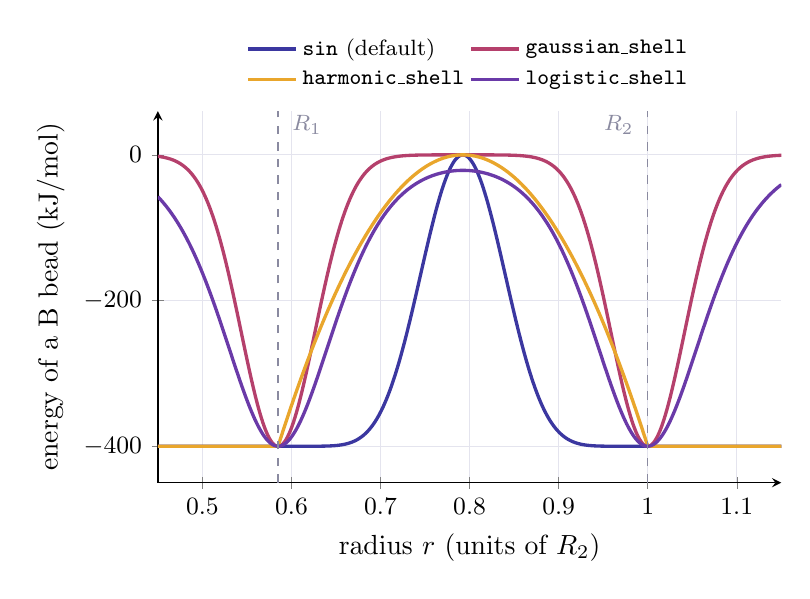
\begin{tikzpicture}
\begin{axis}[xlabel={radius $r$ (units of $R_2$)},ylabel={energy of a B bead (kJ/mol)},
  xmin=0.45,xmax=1.15,ymin=-450,ymax=60,domain=0.45:1.15,samples=400,
  legend style={font=\footnotesize,at={(0.5,1.03)},anchor=south,legend columns=2}]
\addplot[indigo] {400*(sin(deg(pi*(min(max(x,0.585),1)-0.585)/0.415))^8-1)};
\addlegendentry{\texttt{sin} (default)}
\addplot[crimson] {-400*(exp(-(x-0.585)^2/0.003444)+exp(-(x-1)^2/0.003444))};
\addlegendentry{\texttt{gaussian\_shell}}
\addplot[gold] {-400*(min(abs(x-0.7925),0.2075)/0.2075)^2};
\addlegendentry{\texttt{harmonic\_shell}}
\addplot[violet] {-400*(1/cosh(abs(x-0.585)/0.083)^2+1/cosh(abs(x-1)/0.083)^2)};
\addlegendentry{\texttt{logistic\_shell}}
\draw[dashed,grey] (axis cs:0.585,-450) -- (axis cs:0.585,80);
\draw[dashed,grey] (axis cs:1,-450) -- (axis cs:1,80);
\node[font=\footnotesize,grey,anchor=south west] at (axis cs:0.59,15) {$R_1$};
\node[font=\footnotesize,grey,anchor=south east] at (axis cs:0.995,15) {$R_2$};
\end{axis}
\end{tikzpicture}
\end{document}
